\documentclass{ximera}

\prerequisites{geometry}
\outcomes{quadratures}

\graphicspath{{./}{thePythagoreanTheorem/}{deMoivreSavesTheDay/}{complexNumbersFromDifferentAngles/}}

\usepackage{tikz}
\usepackage{tkz-euclide}
\usetkzobj{all}
\tikzstyle geometryDiagrams=[ultra thick,color=blue!50!black]
\newcommand{\tri}{\triangle}
\renewcommand{\l}{\ell}
\renewcommand{\P}{\mathcal{P}}
\newcommand{\R}{\mathbb{R}}
\newcommand{\Q}{\mathbb{Q}}

\newcommand{\Z}{\mathbb Z}

\renewcommand{\vec}{\mathbf}
\renewcommand{\d}{\,d}



%% Egyptian symbols

\usepackage{multido}
\newcommand{\egmil}[1]{\multido{\i=1+1}{#1}{
\includegraphics[scale=.1]{egyptian/egypt_person.pdf}\hspace{0.5mm}}}
\newcommand{\eghuntho}[1]{\multido{\i=1+1}{#1}{
\includegraphics[scale=.1]{egyptian/egypt_fish.pdf}\hspace{0.5mm}}}
\newcommand{\egtentho}[1]{\multido{\i=1+1}{#1}{
\includegraphics[scale=.1]{egyptian/egypt_finger.pdf}\hspace{0.5mm}}}
\newcommand{\egtho}[1]{\multido{\i=1+1}{#1}{
\includegraphics[scale=.1]{egyptian/egypt_lotus.pdf}\hspace{0.5mm}}}
\newcommand{\eghun}[1]{\multido{\i=1+1}{#1}{
\includegraphics[scale=.1]{egyptian/egypt_scroll.pdf}\hspace{0.5mm}}}
\newcommand{\egten}[1]{\multido{\i=1+1}{#1}{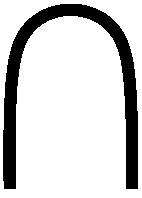
\includegraphics[scale=.1]{egyptian/egypt_heel.pdf}\hspace{0.5mm}}}
\newcommand{\egone}[1]{\multido{\i=1+1}{#1}{
\includegraphics[scale=.1]{egyptian/egypt_stroke.pdf}\hspace{0.5mm}}}
\newcommand{\egyptify}[7]{
 \multido{\i=1+1}{#1}{
\includegraphics[scale=.1]{egyptian/egypt_person.pdf}\hspace{0.5mm}}
 \multido{\i=1+1}{#2}{
\includegraphics[scale=.1]{egyptian/egypt_fish.pdf}\hspace{0.5mm}}
 \multido{\i=1+1}{#3}{
\includegraphics[scale=.1]{egyptian/egypt_finger.pdf}\hspace{0.5mm}}
 \multido{\i=1+1}{#4}{
\includegraphics[scale=.1]{egyptian/egypt_lotus.pdf}\hspace{0.5mm}}
 \multido{\i=1+1}{#5}{
\includegraphics[scale=.1]{egyptian/egypt_scroll.pdf}\hspace{0.5mm}}
 \multido{\i=1+1}{#6}{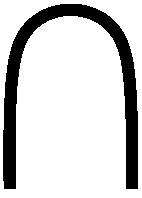
\includegraphics[scale=.1]{egyptian/egypt_heel.pdf}\hspace{0.5mm}}
 \multido{\i=1+1}{#7}{
\includegraphics[scale=.1]{egyptian/egypt_stroke.pdf}\hspace{0.5mm}}
 \hspace{.5mm}
}




\title{Squaring the circle with lunes}
\begin{document}
\begin{abstract}
In this activity we investigate a proposed method of squaring the circle.
\end{abstract}
\maketitle

It is impossible to square the circle with compass and straightedge
alone. However, it is still interesting to think about what one's
strategy might be to achieve this impossible goal. We will work with a
circle of diameter $D$.
\begin{image}
\begin{tikzpicture}[geometryDiagrams]
\draw (0,0) circle (1cm);
\draw[thin] (-1,0)--(1,0);
\node at (0,-.2) {$D$};
\end{tikzpicture}
\end{image}


\begin{question}
Consider a circle of \textbf{radius} $D$. What is the relationship
between the area of the original circle and this new circle?
\end{question}


\begin{question}
Consider a circle of \textbf{radius} $D$. We claim that we can
inscribe a regular hexagon of side length $D$ in this circle.
\begin{image}
\begin{tikzpicture}[geometryDiagrams]
\draw[thin] (0,0) circle (2cm);
\draw (2,0)--({2*cos(60)},{2*sin(60)});
\draw ({2*cos(60)},{2*sin(60)})--({2*cos(120)},{2*sin(120)});
\draw ({2*cos(120)},{2*sin(120)})--({2*cos(180)},{2*sin(180)});
\draw ({2*cos(180)},{2*sin(180)})--({2*cos(240)},{2*sin(240)});
\draw ({2*cos(240)},{2*sin(240)})--({2*cos(300)},{2*sin(300)});
\draw ({2*cos(300)},{2*sin(300)})--(2,0);
\draw[decoration={brace,raise=.2cm},decorate,thin] ({2*cos(120)},{2*sin(120)})--({2*cos(180)},{2*sin(180)});

\node at (-1,.6) {$D$};
\end{tikzpicture}
\end{image}
Explain how you know this is true.
\end{question}


\begin{question}
Still considering a circle of \textbf{radius} $D$, add some lunes.
\begin{image}
\begin{tikzpicture}[geometryDiagrams]
\draw (0,0) circle (2cm);
\draw[thin] (2,0)--({2*cos(60)},{2*sin(60)});
\draw[thin] ({2*cos(60)},{2*sin(60)})--({2*cos(120)},{2*sin(120)});
\draw[thin] ({2*cos(120)},{2*sin(120)})--({2*cos(180)},{2*sin(180)});
\draw[thin] ({2*cos(180)},{2*sin(180)})--({2*cos(240)},{2*sin(240)});
\draw[thin] ({2*cos(240)},{2*sin(240)})--({2*cos(300)},{2*sin(300)});
\draw[thin] ({2*cos(300)},{2*sin(300)})--(2,0);

\draw (2,0) arc (-60:120:1cm);
\draw ({2*cos(60)},{2*sin(60)}) arc (0:180:1cm);
\draw ({2*cos(120)},{2*sin(120)}) arc (60:240:1cm);
\draw ({2*cos(180)},{2*sin(180)}) arc (120:300:1cm);
\draw ({2*cos(240)},{2*sin(240)}) arc (180:360:1cm);
\draw ({2*cos(300)},{2*sin(300)}) arc (-120:60:1cm);
\end{tikzpicture}
\end{image}
Now write two expressions for the area of the entire figure, one built
from the area of a regular hexagon and the area of the original
circle, and the other built from the area of the larger circle and the
area of the lunes.
\end{question}

\begin{question}
Explain how this gives a method for finding the quadrature of a
circle, assuming you know how to find the quadrature of lunes.
\end{question}

\end{document}
